\section{Marco teórico}
\subsection{Aprendizaje automático}
%- explicación resumida tipos de aprendizaje (supervisado, no supervisado, semisupervisado)
 Dentro de las diferentes ramas de la inteligencia artificial, los algoritmos utilizados se pueden clasificar en tres grandes ramas según la forma en que son entrenados: algoritmos de aprendizaje supervisado, algoritmos de aprendizaje semi-supervisado y algoritmos de aprendizaje no supervisado.
 
  Los primeros se utilizan cuando para un conjunto de entrenamiento \(X\) se tiene un conjunto de etiquetas \(y\) relacionadas a elemento; de esta manera, los algoritmos encuadrados dentro de esta rama se encargan de estimar una función que mapee los datos del conjunto \(X\) al conjunto \(y\), con el fin de luego poder realizar inferencias a partir de sólo nuevos casos de entrada.
 
  Los algoritmos de aprendizaje no supervisado se utilizan en situaciones en las que se tiene un conjunto de datos de entrada \(X\) pero no un conjunto de etiquetas asignadas a estos datos, estos algoritmos se emplean para realizar sobre los datos tareas tales como agrupamientos, detección de anomalías, reducción de dimensionalidad, entre otras.
  
  Por último, el aprendizaje semi-supervisado entra en juego en aquellos casos en los que se tiene un pequeño conjunto de datos etiquetado, y un gran conjunto de datos no etiquetados. Existen modelos en los que agregar datos no etiquetados al entrenamiento hace que mejoren sus predicciones, como otros en los que hace que empeoren. Las ideas principales detrás del aprendizaje supervisado son: ayudar a ganar representación general de la población de los datos, y ganar conocimiento sin recurrir a los costos de tiempo y dinero que suponen etiquetar datos que se tienen.
 
%- explicación profunda aprendizaje supervisado, ejemplos otros tipos de problemas
 En este trabajo se contará tanto con un conjunto de entrenamiento (que serán bases de datos de escenas de propiedades) como con sus pertenecientes etiquetas, por lo que se intentará mapear mediante técnicas de aprendizaje profundo cada imagen con sus etiquetas, es decir, se trabajará en un problema de aprendizaje supervisado.
 
 Dentro de esta rama existen otros algoritmos que pueden servir para este problema o para otros de dominio diferente como son los árboles de decisión, regresiones lineales o logísticas, ensembles, etc.
 
\subsection{Representación de una neurona}
%- explicación neurona
 En este trabajo, como bien se explicó anteriormente, se abordará la solución mediante técnicas de aprendizaje profundo, por lo que a continuación se dará lugar a las explicaciones pertinentes relacionadas a este tipo de técnica.
 Para empezar es necesario comentar que el término "profundo" recae en la profundidad de las redes neuronales que se utilizan en esta técnica. Estas redes pueden estar compuestas hasta por millones de neuronas interconectadas entre si; neuronas que se representan como se observa en la imagen \ref{fig:representacion_neurona} donde se muestra un ejemplo con \(n\) entradas, conformada por: 
 \begin{itemize}
 	\item Entradas: conjunto de datos de entrada \(x_1\)..\(x_n\)
 	\item Pesos: conjunto de pesos \(w_1\)..\(w_n\) correspondientes a cada entrada
 	\item Función de agregación: función que sumariza la multiplicación pesada entre cada entrada \(x\) y su correspondiente peso \(w\).
	\item Función de activación: función no lineal responsable de mapear el resultado de la función de agregación en salidas (según que tipo de función sea, los resultados suelen variar entre [0, 1] o [-1, 1]).
	\item Salida: resultado de la función de activación.
 \end{itemize}
 
 
\begin{figure}[!h]
\centering
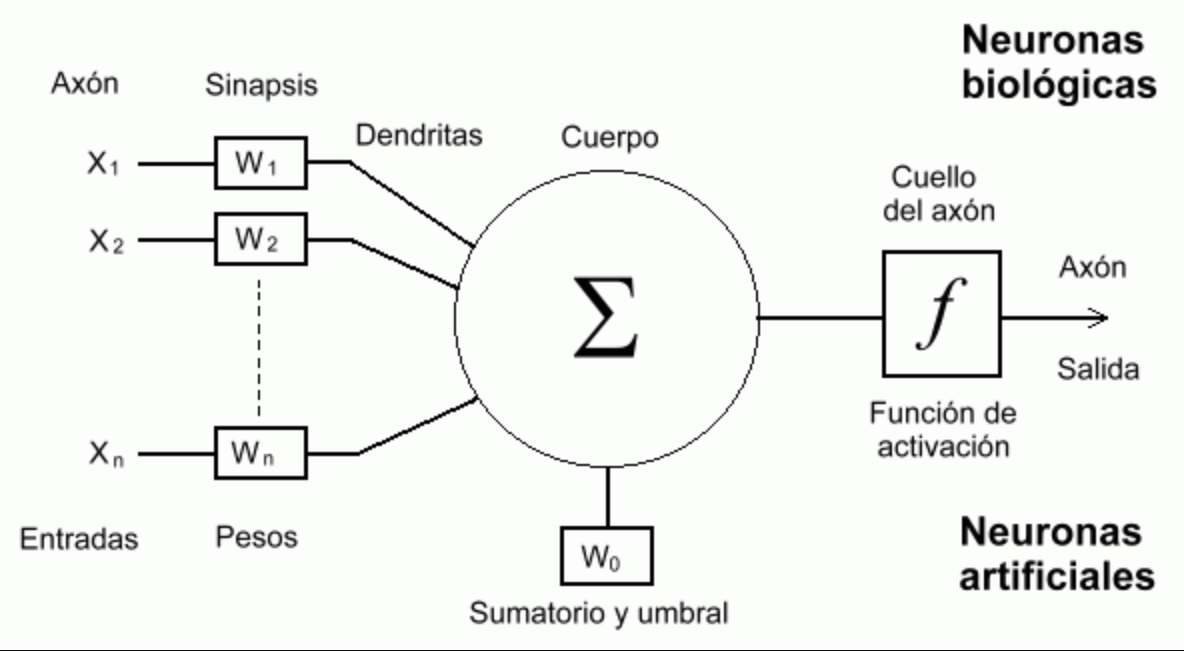
\includegraphics[width=.8\linewidth]{images/representacion_neurona}
\caption[Representación de una neurona]{Representación de una neurona}
\label{fig:representacion_neurona}
\end{figure}

De esta manera, se puede obtener la salida de la neurona \(Y\), a partir de aplicar la función de activación \(\sigma\) a la suma entre el sesgo \(b\) y la multiplicación matricial del conjunto de entradas \(X\) y los pesos \(W\).

\begin{equation}
Y=\sigma\left(W^{T} X+b\right)
\end{equation}


\subsection{Red Neuronal}\label{red_neuronal}
%- explicación redes neuronales profundas
 Una red neuronal, como su nombre lo enuncia, es una consecución de capas de \(N\) neuronas en cada una, conectadas entre sí como se puede ver en el ejemplo de la figura \ref{fig:redneuronal}. Es necesario que se cuente con capas de entrada, ocultas y de salida; para el ejemplo enunciado se cuenta con una capa de entrada, dos capas ocultas y una capa de salida. 
 
 El fin de las redes neuronales es aprender representaciones del contenido de la información en relación a las salidas esperadas para luego poder hacer inferencias en nuevo contenido, a modo de ejemplo, si se tienen imágenes de perros y gatos, y el fin es detectar si se trata de un perro o un gato la red posiblemente no aprenda las mismas representaciones que si el fin de la misma es detectar presencia o ausencia de animales.
 
 
 \begin{figure}[!h]
 	\centering
 	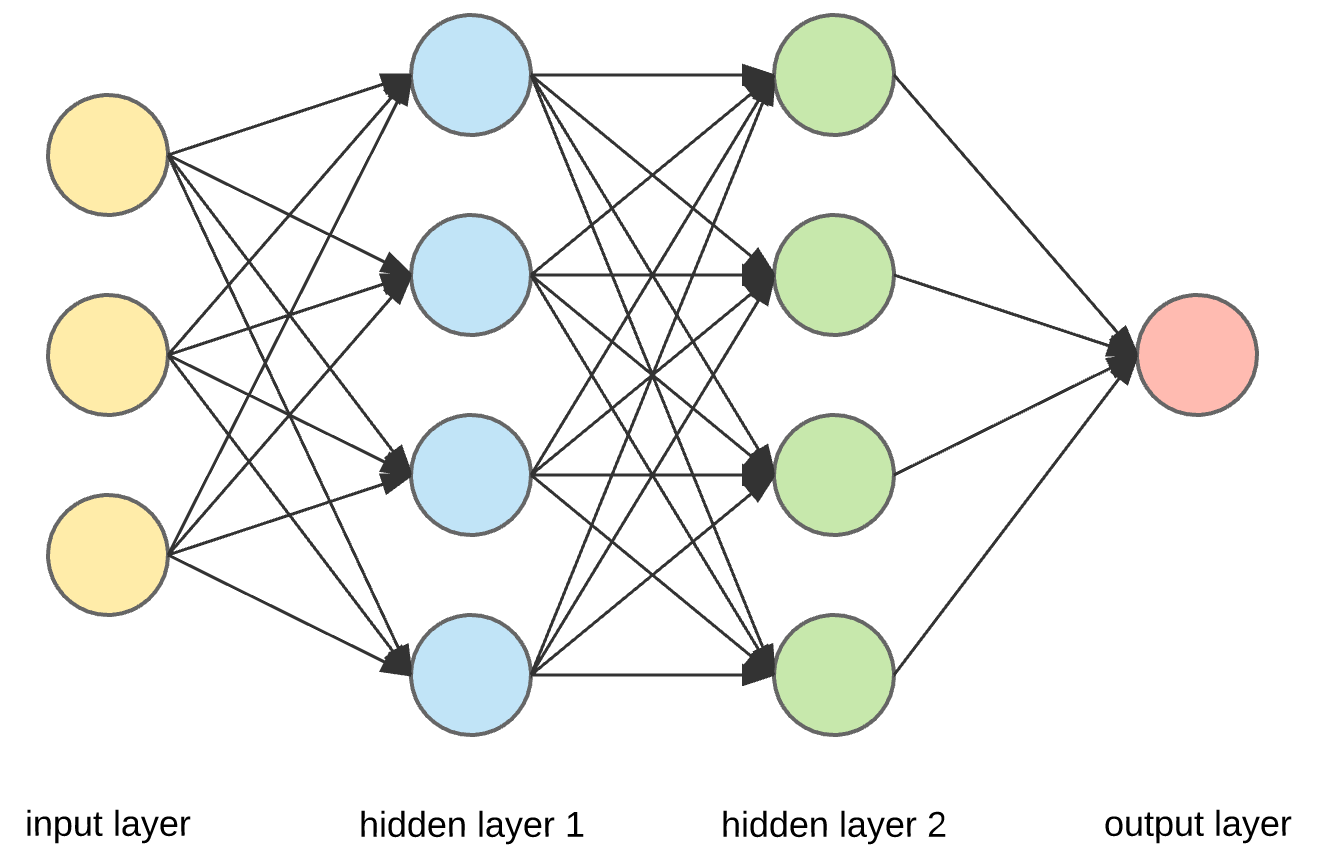
\includegraphics[width=0.7\linewidth]{images/red_neuronal}
 	\caption[Ejemplo red neuronal]{Perceptrón Multi Capa}
 	\label{fig:redneuronal}
 \end{figure}
%- explicacion funcionamiento:

 Para explicar el funcionamiento de las redes neuronales es necesario también introducir algunos conceptos como son la propagación hacia adelante y hacia atrás, función de pérdida y optimización. Durante la fase de entrenamiento, los pasos que se siguen son:
 (i) inicialización de pesos y sesgo, (ii) propagación hacia adelante, (iii) evaluación de función de pérdida y (iv) propagación hacia atrás.
 
 Antes de comenzar a entrenar una red es necesario inicializar los pesos que conectan las capas, suele hacerse se hace de manera aleatoria a partir de una distribución normal, aunque existen otros métodos como hacerlo a partir de una distribución uniforme, la inicialización de Xavier, entre otras.
 
  %	- forward prop 
 La propagación hacia adelante es la actividad en que se le brindan los datos a la capa de entrada de la red para que se evalúen consecutivamente todas las capas siguientes en esa dirección aplicando \ref{formula:forward_prop} en cada una, tomando como entrada la capa inmediata anterior. De esta manera, se obtiene como salida de la red sus predicciones. 
 
 \begin{equation}\label{formula:forward_prop}
 z=W^{T} X+b
 \end{equation}
 
 %	- back prop 
 Luego, a partir de las salidas \(\hat{y}\) de la red es posible medir la función de pérdida (detallado en \ref{formula:loss_function}) que brinda la información de cuán cerca estuvo la red de predecir las salidas correctas y con la que se puede computar la propagación hacia atrás del error, es decir, optimizar la función de pérdida actualizando los pesos desde atrás hacia adelante teniendo en cuenta el error en cada capa. La manera de hacerlo es mediante la derivada parcial de la función de costo con respecto tanto a los pesos \(\omega\) (fórmula \ref{formula:parcial_derivate_w}) como a los sesgos \(b\) (fórmula \ref{formula:parcial_derivate_b}) en cada capa con el fin de obtener un nuevo valor de los pesos y sesgos \(W\) y \(b\) en cada una de éstas.
  
 \begin{equation}\label{formula:loss_function}
 \mathcal{L}(y, \hat{y})=-\sum_{i=1}^{n} y_{i} \log \hat{y}_{i}
 \end{equation}
 
 \begin{equation}\label{formula:parcial_derivate_w}
 \omega =\omega-\alpha \frac{\partial J(\omega, b)}{d \omega}
 \end{equation}
 
 \begin{equation}\label{formula:parcial_derivate_b}
 b=b-\alpha \frac{d J(\omega, b)}{d b}
 \end{equation}
 
%  - loss functions 
%- optimizers
  La función de pérdida se define de diferentes maneras según el problema que se esté tratando, ya sea error cuadrático medio, error absoluto medio, proximidad del coseno, etc. La propuesta general para problemas de clasificación es usar \(entrop{\acute i}a-cruzada\) (o \(cross-entropy\) en inglés), una función derivable que mide qué tan lejos del resultado esperado están las salidas de la red, como se observa en la ecuación \ref{formula:loss_function}. Como se mencionó anteriormente, el objetivo de la red es minimizar la función de pérdida y para esto se requiere de una función de optimización. \(Adam\), introducido en \cite{kingma2014adam} es un optimizador en que se puede tener ciertas certezas de su correcto funcionamiento ya que su implementación tiene en cuenta las principales mejoras de otros como son el Descenso por el Gradiente con Momentum y la Propagacion de la Raíz Cuadrada de la Media de los Cuadrados.
  
%	- regularizers:
 %		- dropout
 %		- batch norm
 Un problema común al entrenar una red es el sobreentrenamiento, que se da cuando la red sobreajusta sus pesos para el conjunto de entrenamiento y pierde capacidad de generalizar. Una forma fácil de controlarlo es mediante la verificación de la función de pérdida y las métricas elegidas sobre un subconjunto de validación, que son imágenes que no se utilizan para entrenar la red sino que para medir cómo está funcionando la misma (si la red está sobreentrenando, entonces la diferencia entre las métricas de entrenamiento y validación comenzarán a incrementarse, siendo las de entrenamiento mayores a las otras). Para contrarrestar estas situaciones existen capas regularizadoras, es decir, que evitan la concetración de gran porcentaje del conocimiento en un subconjunto de unidades en las capas y por ende el aprendizaje de la representación del contenido sea compartido entre las neuronas de las capas. Aunque existen otras, las más utilizadas son \(dropout\) y \(batch-normalization\). La capa \(dropout\) se encarga de apagar conexiones aleatoriamente entre capas durante el entrenamiento, esto hace que no se entrene siempre con las mismas unidades dentro de cada capa, y así, que no sean siempre las mismas neuronas las que se activen frente a cada situación. La capa de \(batch-normalization\) aplica una función de regularización que sale de la media y la varianza de cada sampleo durante el entrenamiento, agregando ruido en las activaciones y evitando que las mismas no sean demasiado altas ni bajas, reduciendo de esta manera el desplazamiento covariable interno (\(internal\;covariance\; shift\), en inglés), y la manera de hacerlo es mediante la aplicación de las ecuaciones \ref{formula:bn_minibatch_mean}, \ref{formula:bn_minibatch_variance}, \ref{formula:bn_normalization}, \ref{formula:bn_scale_and_shift}, como se explica en el Algoritmo 1 de \cite{BatchNorm}.
 
 
 \begin{equation}\label{formula:bn_minibatch_mean}
 \mu_{\mathcal{B}} = \frac{1}{m} \sum_{i=1}^{m} x_{i}
\quad { // media\; del \; mini-batch}
 \end{equation}
 
 \begin{equation}\label{formula:bn_minibatch_variance}
 \sigma_{\mathcal{B}}^{2} = \frac{1}{m} \sum_{i=1}^{m}\left(x_{i}-\mu_{\mathcal{B}}\right)^{2}
\quad { // varianza \; del \; mini-batch}
 \end{equation}
 
 \begin{equation}\label{formula:bn_normalization}
 \widehat{x}_{i} = \frac{x_{i}-\mu_{\mathcal{B}}}{\sqrt{\sigma_{\mathcal{B}}^{2}+\epsilon}}
\quad { // normalizacion}
 \end{equation}
 
 \begin{equation}\label{formula:bn_scale_and_shift}
 y_{i} = \gamma \widehat{x}_{i}+\beta \equiv \mathrm{B} \mathrm{N}_{\gamma, \beta}\left(x_{i}\right) {// escalacion \; y \; desplazamiento}
 \end{equation}
 
%- activation functions
 Las capas convolutivas y las capas totalmente conectadas requieren de una función de activación para determinar su salida, y aunque existe gran variedad de estas, hay algunas funciones que se sabe que funcionan bien ante determinados problemas. A continuación se detallarán algunas de las funciones de activación que posiblemente se utilicen a en las etapas de experimentación:
 \begin{itemize}
 	\item Sigmoide (\(Sigmoid\)): Está definida como \ref{formula:activations_sigmoid} y la razón principal por la que se la utiliza es debido a que sólo devuelve valores entre [0, 1], por lo que es muy útil en tareas en las que se necesita predecir la probabilidad de una clase. 
 	\begin{equation}\label{formula:activations_sigmoid}
 	\sigma(x)=\frac{1}{1+e^{-x}}
 	\end{equation}
 	\begin{figure}[!ht]
 		\centering
 		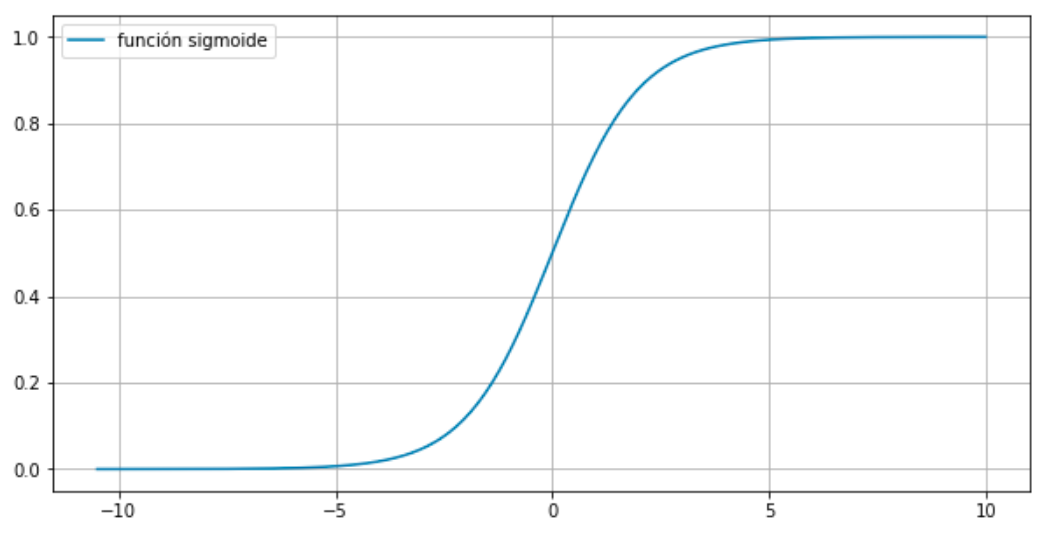
\includegraphics[width=0.7\linewidth]{images/activations_sigmoid}
 		\caption[Función Sigmoide]{Función Sigmoide}
 		\label{fig:sigmoid}
 	\end{figure}
 	
 	\item Tangente hiperbólica (\(TanH\)): Su formulación se explicita en \ref{activations_tanh}. Como se puede observar en la figura \ref{fig:activationstanh}, mantiene la forma S de la función Sigmoide pero en este caso los resultados posibles van desde [-1, 1]. 
 	\begin{equation}
\label{activations_tanh}
 	\tanh (x)=\frac{2}{1+e^{-2 x}}-1
 	\end{equation}
 	\begin{figure}[!h]
 		\centering
 		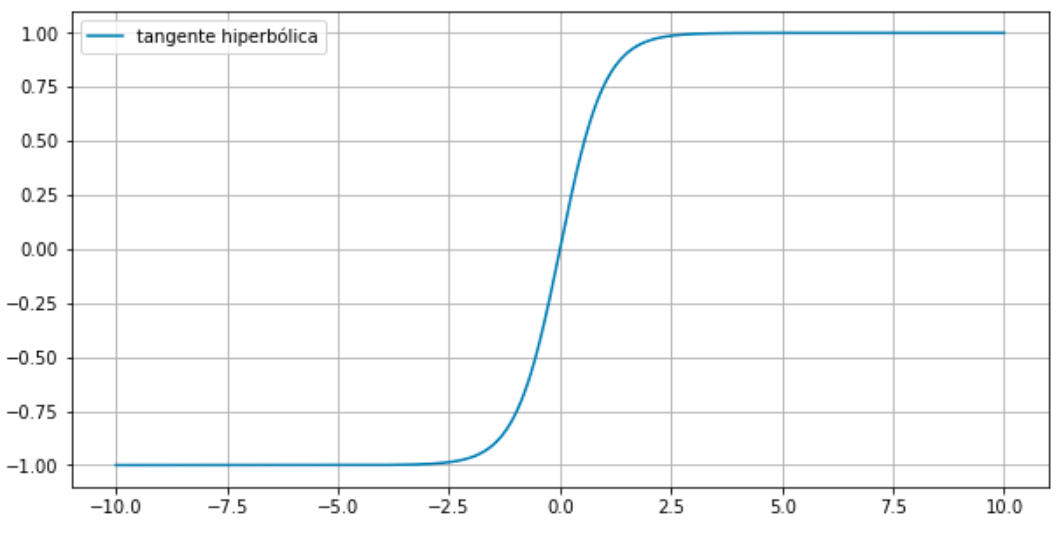
\includegraphics[width=0.7\linewidth]{images/activations_tanh}
 		\caption[Función Tangente Hiperbólica]{Función Tangente Hiperbólica}
 		\label{fig:activationstanh}
 	\end{figure}
 	 	 	
 	\item Unidad lineal rectificada (\(ReLu\)): En la figura \ref{fig:activationsrelu} se puede observar el comportamiento de esta función (definida en la fórmula \ref{activations_relu}), en donde para valores negativos el resultado es cero, mientras que para el resto, el resultado es el mismo valor. Por este comportamiento es una de las funciones de activación más utilizadas (junto a sus otras variantes eLu, LeakyReLu, etc) en las capas ocultas de las redes neuronales.
 	\begin{figure}[!h]
 		\centering
 		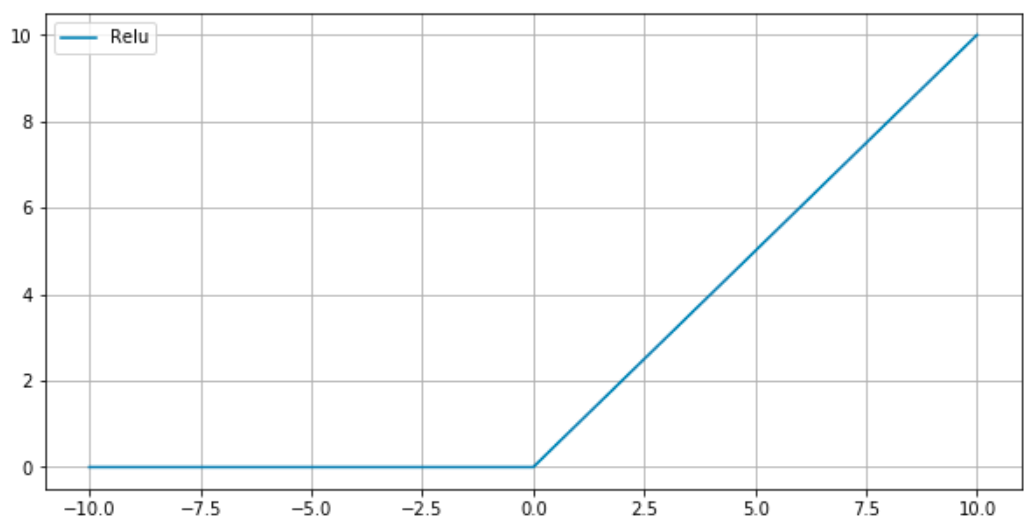
\includegraphics[width=0.7\linewidth]{images/activations_relu}
 		\caption[Función ReLu]{Función ReLu}
 		\label{fig:activationsrelu}
 	\end{figure}
 	\begin{equation}\label{activations_relu}
 	ReLu(x)=\max (0, x)
 	\end{equation}
	\item\label{item:softmax} Exponencial normalizada (\(Softmax\)): es una variante de la función Sigmoide pero definida para problemas de clasificación multiclase; como se observa en la fórmula \ref{activations_softmax}, normaliza las entradas en una salida que es en un vector de \(K\) valores de probabilidad (uno por cada clase definida) entre [0, 1] que sumados dan uno.
	\begin{equation}
\label{activations_softmax}
	\sigma(\mathbf{z})_{j}=\frac{e^{z_{j}}}{\sum_{k=1}^{K} e^{z_{k}}} \quad \text { por cada } j=1, \ldots, K
	\end{equation}
	Siendo \(K\) la cantidad de clases.
 \end{itemize}

	
\subsection{Red Neuronal Convolucional}
%- explicación razón de convoluciones
Las redes neuronales convolucionales son una variante de las redes neuronales en las que la extracción de características se realiza mediante capas convolucionales. Fueron introducidas en \cite{lecun1995convolutional} por LeCun y Bengio, investigadores referentes en el mundo del aprendizaje automático y las redes neuronales, y han transformado la forma de resolver problemas de clasificación de imágenes (y otros ) desde entonces.

Como es posible observar en la figura \ref{fig:convolution}, una convolución es una operación matemática. Se puede entender como el resultado de aplicar un filtro (una matriz con forma \(N x N\)) en todas las regiones de la imagen con el fin de obtener una nueva.
\begin{figure}[!h]
	\centering
	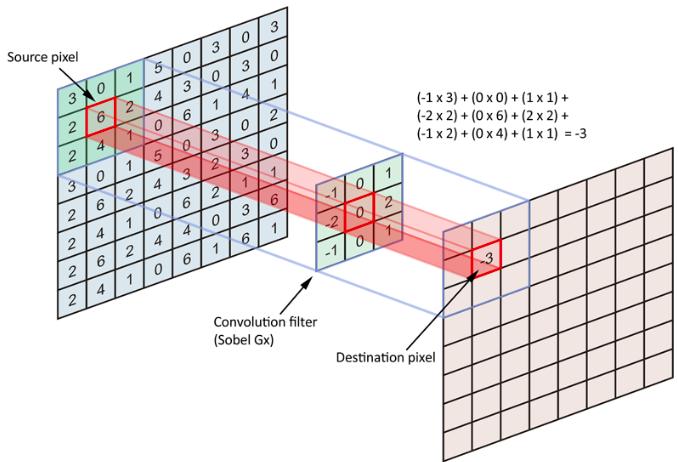
\includegraphics[width=0.7\linewidth]{images/convolution}
	\caption[Convolución]{Convolución}
	\label{fig:convolution}
\end{figure}

\begin{equation} \label{formula:sample_filter}
\begin{split}
f & = (-1 * 3) + (0 * 0) + (1 * 1) \\
& + (-2 * 2) + (0 * -6) + (2 * 2)\\
& + (-1 * 2) + (0 * 4) + (1 * 1) = -3 
\end{split}
\end{equation}

 En el ejemplo se aprecia que el resultado de la aplicación del filtro en la esquina superior izquierda de la imagen se obtiene a partir de multiplicar cada valor del pixel en la imagen de entrada con su par en la misma posición en el filtro, finalmente en el ejemplo se tiene que el valor del nuevo pixel en la imagen de salida se obtiene como se observa en la formulación \ref{formula:sample_filter}. La operación detallada previamente se aplica a toda la imagen para obtener la imagen resultado, teniendo en cuenta tanto los valores del \(stride\) como del \(padding\) definidos para la capa.
 
 El parámetro \(stride\) define cada cuántos píxeles de la imagen de entrada se aplicará el filtro, mientras que mediante el parámetro \(padding\) se decide cómo se tratarán los bordes, esto es debido a que existen ocasiones en las que se desea obtener una imagen en la que se le apliquen convoluciones también a los bordes de la misma; las formas más comunes de hacerlo son agregando a los bordes \(N\)) pixeles más (dependiendo del \(stride\)), ya sea imputándolos como ceros o con mismo valor de sus píxeles más cercanos. 
 
Gracias a estas capas las redes convolucionales son capaces de aprender representaciones del contenido invariantes, ya que cada filtro se aplica a todas las subregiones de la imagen haciendo que el aprendizaje obtenido en las capas más profundas se base en las imágenes completas. A continuación se detallará cómo funciona una red convolucional, con el fin de mostrar cómo estas las capas convolutivas se interconectan entre sí, reducen las representaciones computadas y finalmente se conectan con capas totalmente conectadas para realizar inferencia a partir de lo aprendido.

\begin{figure}
	\centering
	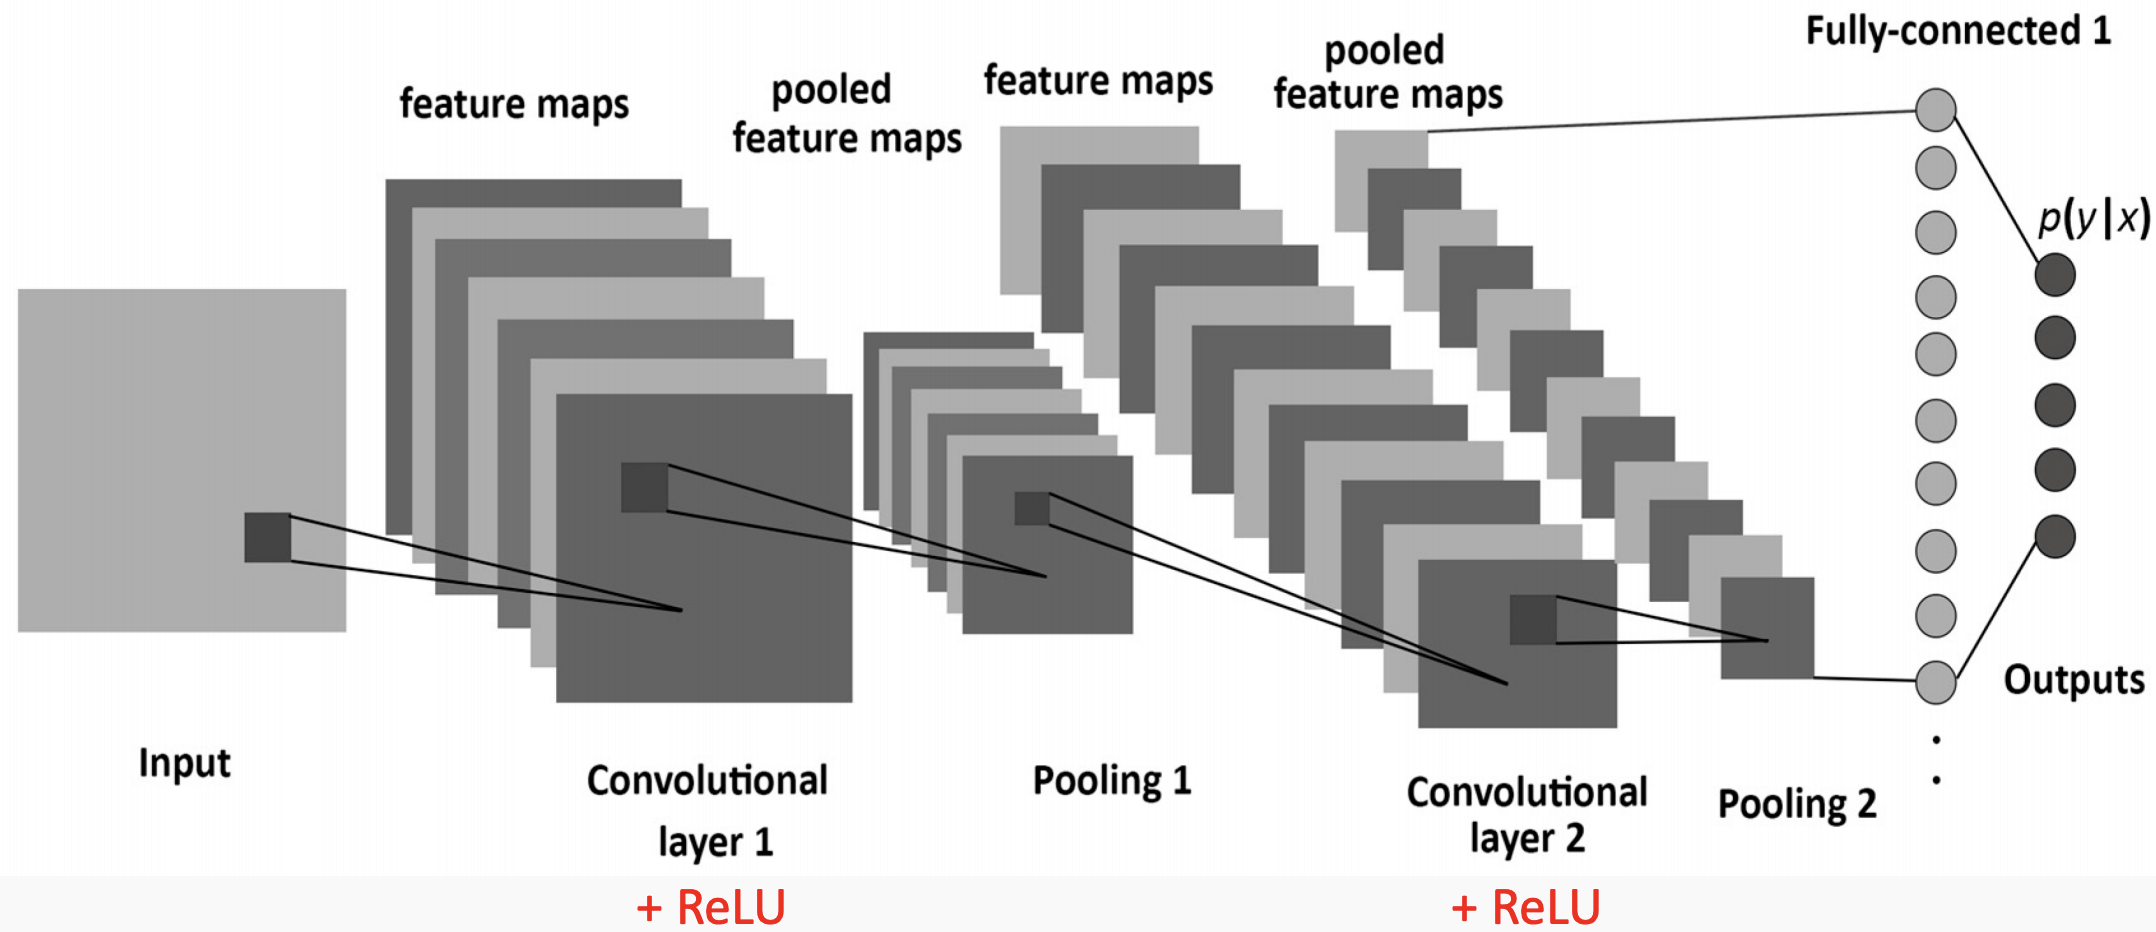
\includegraphics[width=0.75\linewidth]{images/cnn_explanation}
	\caption[Ejemplo Red Neuronal Convolucional]{Ejemplo Red Neuronal Convolucional}
	\label{fig:cnnexplanation}
\end{figure}

Existen muchas configuraciones de redes neuronales convolucionales, aunque para simplificar la explicación se utilizará una red compuesta de la siguiente manera: capa convolucional, capa de pooling, capa convolucional, capa de pooling, capa totalmente conectada y capa de salida (ilustrada en la figura \ref{fig:cnnexplanation}). La capa de entrada en este caso (al igual que en el presente trabajo) serán imágenes en formato RGB normalizadas, es decir, una matriz de \([alto \; x \;ancho \;x \;n. \;canales]\) por cada imagen; luego esta entrada será convolucionada aplicando la operación matemática previamente explicada y sus salidas serán agrupadas por una capa llamada \(pooling\). En esta capa se buscará reducir tanto las representaciones aprendidas como la cantidad de cálculos a realizar: se agruparán mediante la aplicación de un filtro \(f\) y un método \(M\) los resultados de la convolución, siendo \(f\) una matriz (usualmente de \([2\;x\; 2]\)) y \(M\) la utilización de la media o el máximo de los valores de la imagen en cada sector en que se aplique el filtro; al igual que en la convolución, la operación de pooling se aplica en toda la imagen, aunque tiene dos diferencias fundamentales: no tiene parámetros que aprender o ajustar y busca reducir las representaciones a matrices de menor orden. Continuando con la red, se aplica nuevamente una convolución seguida de una capa de pooling que se conecta a una capa totalmente conectada (la misma que se utiliza en el perceptrón multicapa). 
%Antes de llegar a la capa de predicciones, la capa totalmente conectada se conecta a una de dropout que se encarga de apagar conexiones entre neuronas de dos capas contiguas aleatoriamente durante el entrenamiento con el fin de ayudar a que el conocimiento no quede sólo en algunas de éstas. 
Finalmente, la capa de totalmente conectada se conecta con una capa de salida que se encargará de computar las probabilidades con las que se predice cada clase (básicamente, otra capa totalmente conectada con función de activación Softmax, mencionada en \ref{item:softmax}).

\subsection{Redes preentrenadas y Aprendizaje por transferencia} 

% Redes preentrenadas
Como entrenar redes neuronales profundas resulta muy costoso computacionalmente tanto por la profundidad de las mismas como por la cantidad de datos con las que se las necesita entrenar, con el pasar del tiempo quienes tienen accesso a capacidad de cómputo comenzaron a liberar redes entrenadas con diferentes bases de datos. Posiblemente, las redes liberadas más conocidas sean las que se entrenaron utilizando ImageNet \cite{ImageNet}, una base de datos de 3.2 millones imágenes centradas en objetos, aunque también existen otras redes preentrenadas con otras bases de datos de imágenes abiertas como son COCO Dataset \cite{BMVC2015_52}, Places Dataset \cite{learning_deep_features}, etc.


\begin{figure}[!h]
	\centering
	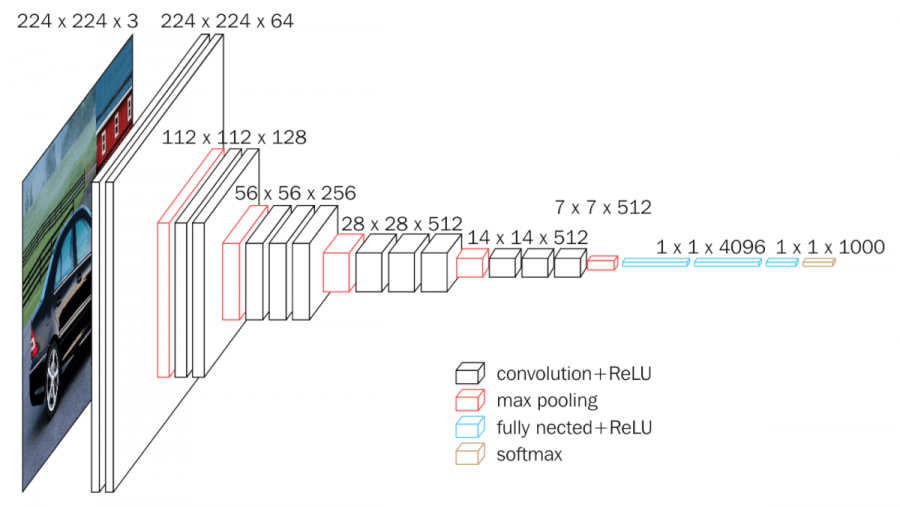
\includegraphics[width=1\linewidth]{images/vgg16}
	\caption[Arquitectura VGG16]{Arquitectura VGG16}
	\label{fig:vgg16}
\end{figure}

%- Transfer Learning
En la actualidad existen redes con diferentes arquitecturas preentrenadas utilizando diversos conjuntos de datos como son VGGNet (figura \ref{fig:vgg16}), InceptionNet (figura \ref{fig:googlenet}), DenseNet, ResNet, Bert, GPT2. Dependiendo el tipo de problema y la base de datos con la que fue entrenada cada red, es posible tomar provecho de las mismas mediante un método llamado \(Aprendizaje\) \(por\; transferencia\) (o \(Transfer\;Learning\) en inglés). 

La forma más simple de utilizar estas redes para hacer transferencia de aprendizaje es haciendo inferencia directamente a partir de ellas, es decir, luego de descargarlas, brindarles datos de entrada y realizar una pasada hacia adelante con el fin de obtener las salidas, aunque la única sitaución para hacerlo es si la red fue preentrenada con el mismo objetivo que el problema en cuestión (no se puede cambiar de un problema de clasificación binaria a uno multiclase directamente). Otra opción es reentrenar a la red con un conjunto de datos propio, de manera de extraer las características aprendidas por la misma y poder refinar sus pesos con un conjunto de entrenamiento que se entiende será más similar a lo que luego se utilizará para realizar predicciones. Por último, otra alternativa es reentrenar estas redes es quitando la capa de salida y agregando capas conectadas a la anteúltima capa de la red. Esto permite tanto agregar capas extra sin entrenar a la red como cambiar las predicciones esperadas utilizando una capa de salida diferente a la inicial.

\begin{figure}
	\centering
	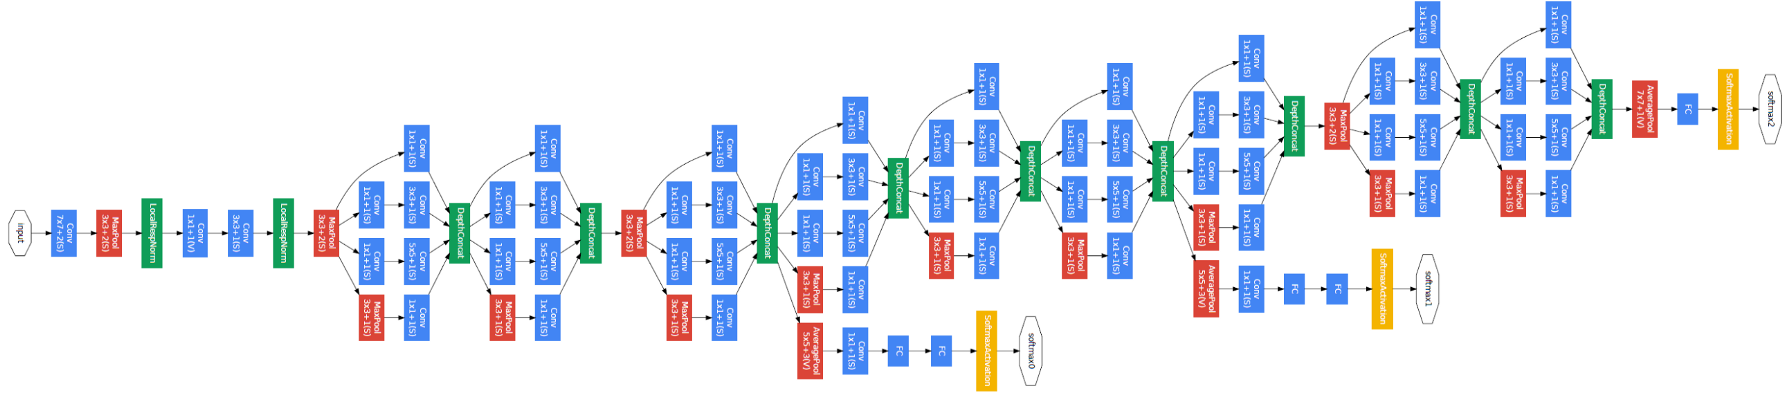
\includegraphics[width=1\linewidth]{images/googlenet}
	\caption[Arquitectura InceptionNet]{Arquitectura InceptionNet}
	\label{fig:googlenet}
\end{figure}